\begin{figure}[htbp]
    \centering
    %
    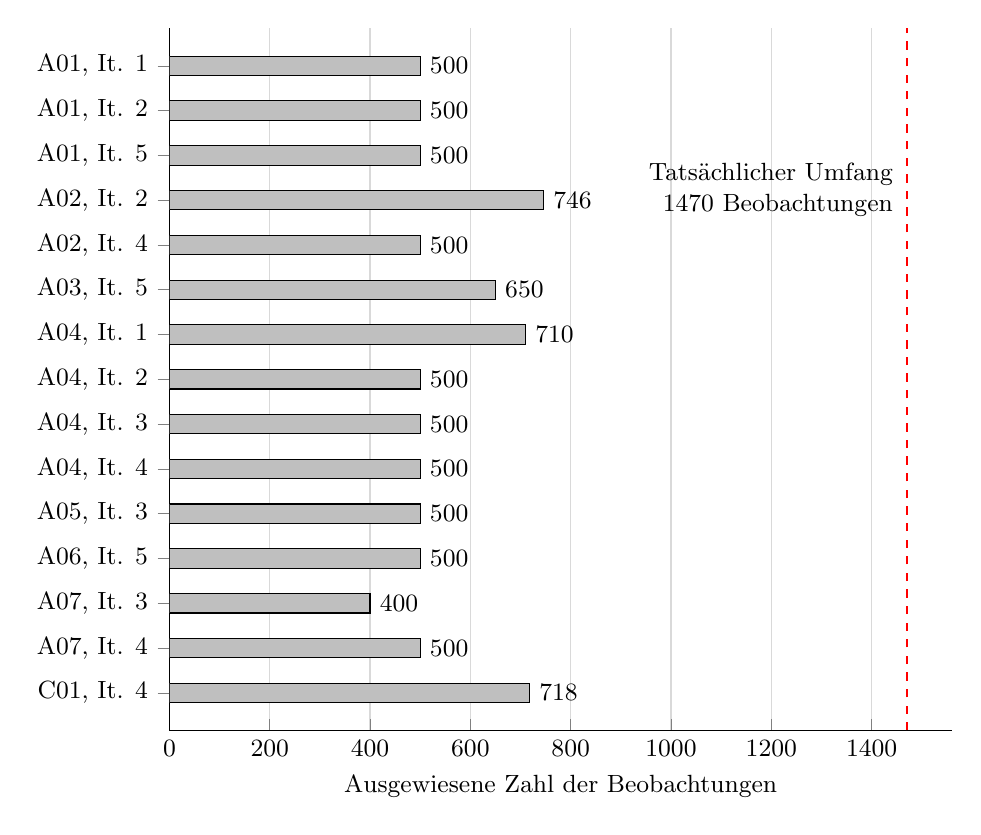
\begin{tikzpicture}
    \begin{axis}[
        width=0.95\textwidth,
        height=10.5cm,
        %
        xbar,
        bar width=7pt,
        %
        xmin=0,
        xmax=1560,
        %
        xtick={0,200,400,600,800,1000,1200,1400},
        scaled x ticks=false,
        %
        x tick label style={
            font=\small,
            /pgf/number format/1000 sep={}
        },
        %
        xlabel={Ausgewiesene Zahl der Beobachtungen},
        xlabel style={font=\small},
        %
        symbolic y coords={
            c15,c14,c13,c12,c11,c10,c9,c8,c7,c6,c5,c4,c3,c2,c1
        },
        %
        ytick=data,
        %
        yticklabels={
            {A01, It. 1},
            {A01, It. 2},
            {A01, It. 5},
            {A02, It. 2},
            {A02, It. 4},
            {A03, It. 5},
            {A04, It. 1},
            {A04, It. 2},
            {A04, It. 3},
            {A04, It. 4},
            {A05, It. 3},
            {A06, It. 5},
            {A07, It. 3},
            {A07, It. 4},
            {C01, It. 4}
        },
        %
        tick label style={font=\small},
        %
        enlarge y limits=0.06,
        %
        xmajorgrids=true,
        grid style={draw=black!15},
        %
        axis lines*=left,
        %
        nodes near coords,
        nodes near coords style={
            font=\small,
            /pgf/number format/1000 sep={}
        }
    ]
    %
    % Von Gemini ausdrücklich genannte Beobachtungszahlen
    \addplot[
        draw=black,
        fill=black!25
    ] coordinates {
        (500,c1)
        (500,c2)
        (500,c3)
        (746,c4)
        (500,c5)
        (650,c6)
        (710,c7)
        (500,c8)
        (500,c9)
        (500,c10)
        (500,c11)
        (500,c12)
        (400,c13)
        (500,c14)
        (718,c15)
    };
    %
    % Tatsächliche Datensatzgröße
    \draw[dashed, thick, red]
        ({axis cs:1470,c1}|-{rel axis cs:0,0})
        --
        ({axis cs:1470,c1}|-{rel axis cs:0,1});
    %
    % Beschriftung der Referenzlinie
    \node[
        anchor=south east,
        font=\small,
        align=right,
        inner sep=3pt
    ]
        at ({axis cs:1460,c1}|-{rel axis cs:0,0.72})
        {Tatsächlicher Umfang\\1470 Beobachtungen};
    %
    \end{axis}
    \end{tikzpicture}
    %
    \caption[Ausgewiesene Beobachtungszahlen]{
        Von Gemini ausgewiesene Beobachtungszahlen im Vergleich zur
        tatsächlichen Größe des übergebenen Datensatzes. Aufgeführt sind
        alle Antworten, in denen der Umfang der zugrunde gelegten
        Datengrundlage ausdrücklich genannt wird, jeweils mit Frage und
        Iteration.
    }
    \label{fig:beobachtungszahlen}
\end{figure}